\documentclass[11pt]{article}
\usepackage[margin=0.85in]{geometry}
\usepackage{amsmath,amssymb,amsthm}
\usepackage{graphicx}
\usepackage{hyperref}

\newtheorem{theorem}{Theorem}
\newcommand{\R}{\mathbb R}
\newcommand{\Ptwo}{\mathcal P_2}

\title{No Uniform Wasserstein Convexity Modulus for Vanishing MMD Regularization}
\author{Run \texttt{fa\_banach\_001}, lane 0}
\date{2026-07-21}

\begin{document}
\maketitle

\section*{Status}

\textbf{Candidate counterexample, likely valid; full negative answer in the
stated generality.}  We give standard admissible data for which every
generalized-geodesic convexity modulus tends to minus infinity as the MMD
regularization parameter tends to zero.

\section*{Source Question}

Stein, Neumayer, Rux, and Steidl ask in Remark 23 of
\emph{Wasserstein Gradient Flows for Moreau Envelopes of $f$-Divergences in
Reproducing Kernel Hilbert Spaces}, arXiv:2402.04613 \cite{SNRS}, whether the
functionals $D_{f,\nu}^{\lambda_N}$, with $\lambda_N\downarrow0$, have a
uniform lower bound on their convexity moduli along generalized geodesics.
Such a bound would permit direct application of a stability theorem for
Wasserstein gradient flows.

\begin{center}

\includegraphics[width=0.98\linewidth]{figures/open_question_crop.png}
\end{center}

We use the source's convention: a functional $E$ is $\kappa$-convex along
generalized geodesics if the appropriate generalized geodesic
$\gamma_{\boldsymbol\alpha,t}$ satisfies
\[
 E(\gamma_{\boldsymbol\alpha,t})
 \le (1-t)E(\mu)+tE(\eta)
 -\frac{\kappa}{2}t(1-t)W_{\boldsymbol\alpha}^2(\mu,\eta).
\]

\section*{Counterexample}

\begin{theorem}\label{thm:main}
Let $d=1$, let
\[
 K(x,y)=\exp\!\left(-\frac{(x-y)^2}{2}\right),
 \qquad f(a)=(a-1)^2\quad(a\ge0),
 \qquad \nu=\delta_0,
\]
where $f=+\infty$ on $(-\infty,0)$.  Put
$E_\lambda=D_{f,\delta_0}^{\lambda}$ for $\lambda>0$.
If $E_\lambda$ is $\kappa_\lambda$-convex along generalized geodesics, then
\[
 \kappa_\lambda
 \le -\frac{1}{e\lambda(1+2\lambda)}.
\]
In particular, if $\lambda_N\downarrow0$, there is no finite uniform lower
bound for the moduli $\kappa_{\lambda_N}$.
\end{theorem}

\begin{proof}
The function $f$ is the standard Tsallis--2 entropy and has infinite recession
constant.  Therefore, for target $\delta_0$, a nonnegative measure $\sigma$
has finite $D_f(\sigma\mid\delta_0)$ only if $\sigma=a\delta_0$ for some
$a\ge0$.  For $c=K(x,0)=e^{-x^2/2}$, the definition of the non-tight
regularization gives
\begin{align*}
 H_\lambda(x):=E_\lambda(\delta_x)
 &=\min_{a\ge0}\left\{(a-1)^2+
       \frac{1+a^2-2ac}{2\lambda}\right\}.
\end{align*}
The unique unconstrained minimizer is
\[
 a_\lambda(x)=\frac{2\lambda+c}{2\lambda+1}>0,
\]
so it also solves the constrained problem.  Substitution yields
\begin{align}
 H_\lambda(x)
 &=\frac{(1-c)(c+4\lambda+1)}{2\lambda(1+2\lambda)} \label{eq:H}\\
 &=\frac{1-e^{-x^2}}{2\lambda(1+2\lambda)}
   +\frac{2(1-e^{-x^2/2})}{1+2\lambda}. \notag
\end{align}
The source records the same Dirac/Tsallis--2 computation in Remark 27:
\begin{center}
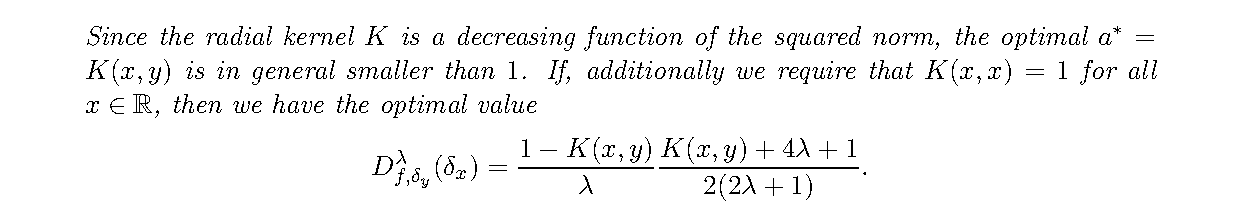
\includegraphics[width=0.94\linewidth]{figures/source_tsallis2_formula_crop.png}
\end{center}

For $g_a(x)=1-e^{-ax^2}$,
\[
 g_a''(x)=2a e^{-ax^2}(1-2ax^2).
\]
At $x=1$ this gives $g_1''(1)=-2/e$ and
$g_{1/2}''(1)=0$.  Hence \eqref{eq:H} implies
\begin{equation}\label{eq:curvature}
 H_\lambda''(1)=-\frac{1}{e\lambda(1+2\lambda)}.
\end{equation}

It remains to relate this one-dimensional curvature to generalized
Wasserstein geodesics.  Fix \mbox{$h>0$} and take endpoints
$\delta_{1-h}$ and $\delta_{1+h}$.  In every three-plan defining a generalized
geodesic between these endpoints, the second and third coordinates are fixed.
Consequently the generalized geodesic is necessarily
\[
 t\longmapsto\delta_{1+(2t-1)h},
 \qquad W_{\boldsymbol\alpha}^2=4h^2,
\]
independently of its base.  Applying $\kappa_\lambda$-convexity at $t=1/2$
gives
\[
 H_\lambda(1+h)+H_\lambda(1-h)-2H_\lambda(1)
 \ge \kappa_\lambda h^2.
\]
After division by $h^2$ and passage to $h\downarrow0$, equation
\eqref{eq:curvature} gives
\[
 \kappa_\lambda\le H_\lambda''(1)
 =-\frac{1}{e\lambda(1+2\lambda)}.
\]
The right-hand side tends to $-\infty$ as $\lambda\downarrow0$.
\end{proof}

\section*{The Source's Approximation Hypotheses Still Hold}

This obstruction is compatible with the exact setup of Remark 23.  Set
\[
 \lambda_N=\frac1N,\qquad
 \mu_0=\delta_0,\qquad
 \mu_{0,N}=\frac1N\sum_{i=1}^N\delta_0=\delta_0.
\]
The initial measures are empirical, converge to $\mu_0$, and satisfy
\[
 \sup_N D_{f,\delta_0}^{\lambda_N}(\mu_{0,N})=0.
\]
Nevertheless, Theorem~\ref{thm:main} forces every valid global modulus to
obey
\[
 \kappa_{\lambda_N}\le -\frac{N}{e(1+2/N)}\longrightarrow-\infty.
\]
Thus the requested uniform lower bound does not exist even when all the
energy and empirical-approximation assumptions in the source remark are met.

\section*{Scope and Interpretation}

The theorem answers the source's question negatively under its general
assumptions.  It does not assert that these gradient flows fail to converge:
for the particular initial data above the flows are stationary.  What fails
is the proposed global uniform-semiconvexity route to convergence.  Uniform
bounds under additional restrictions---for example non-atomic targets,
selected entropy/kernel classes, or along controlled trajectories---are not
addressed here.

\section*{Verification and Novelty Bounds}

The scalar minimization and the value of $H_\lambda''(1)$ were independently
checked symbolically.  The full algebra is recorded in
\texttt{verification.md}.  The cheap run indexes contain no prior entry for
arXiv:2402.04613 or for this Gaussian/Tsallis--2 curvature obstruction.
Bounded arXiv searches on 2026-07-21 found the source and related MMD-flow
papers, but no later explicit resolution of this uniform-modulus question.

\begin{thebibliography}{9}
\bibitem{SNRS}
V. Stein, S. Neumayer, N. Rux, and G. Steidl.
\emph{Wasserstein Gradient Flows for Moreau Envelopes of $f$-Divergences in
Reproducing Kernel Hilbert Spaces}.
arXiv:2402.04613, 2024; revised 2025.
\href{https://arxiv.org/abs/2402.04613}{arXiv:2402.04613}.
\end{thebibliography}

\end{document}
